
\section{Programmierschnittstellen}\label{Appendix:Programmierschnittstellen}

\subsection{Geräte-Manager}\label{Appendix:Geraete_Manager}

\begin{figure}[H]
\center
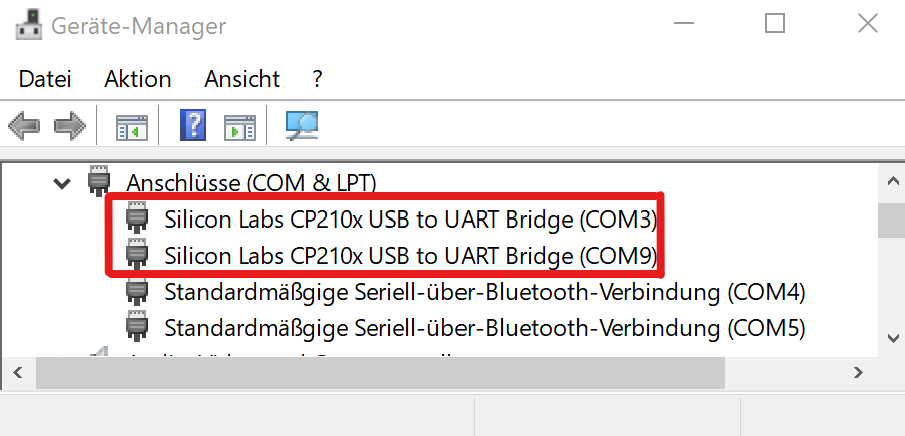
\includegraphics[width = 0.6 \textwidth]{graphics/USB_Devices_Ger_Man}
\caption{Geräte-Manager mit den aufgelisteten USB-UART-Converter (Mikrocontroller und WiFi-Modul).}
\label{fig:USB_Devices_Ger_Man}
\end{figure}

\subsection{Atmega2560}\label{Appendix:Handshake_uC}

\subsubsection{Wiring}\label{Appendix:Handshake_uC_wiring}

\begin{table}[H]
\center
\begin{tabular}{|c|lcl|c|}
\hline
\textbf{Mikrocontroller} & & & & \textbf{USB-Flash-Device} \\ \hline
RX & <== & direkt & === & TX  \\
TX & === & direkt & ==> & RX  \\
Reset & <== & Kondensator & === & DTR \\
\hline
\end{tabular}
\caption{Verbindung zwischen USB und Mikrocontroller.}
\label{tab:USB_uC}
\end{table}

\subsubsection{Handshake}\label{Appendix:Handshake_uc_Messung}
\begin{figure}[H]
\center
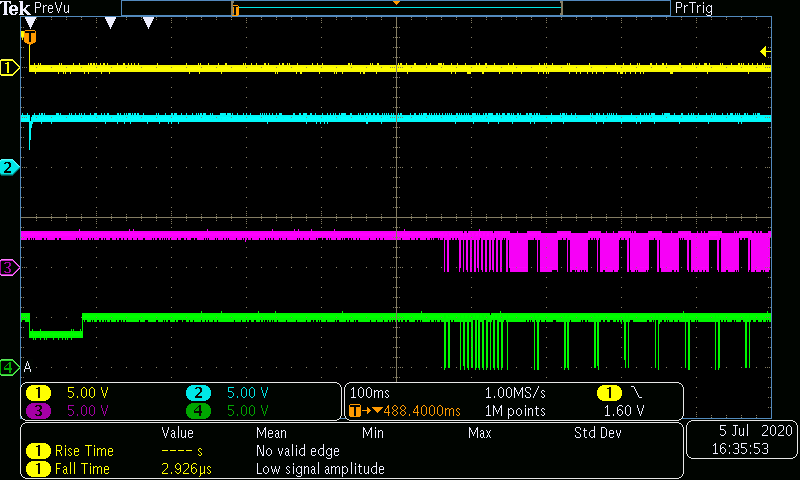
\includegraphics[width = \textwidth]{graphics/ATMega2560_DTR_RESET_RX_TX_gesamt}
\caption{Hochladen des Programmcodes auf den ATMega2560.\\\hspace{\textwidth}1: Gelb = DTR; 2: Blau = Reset; 3: Violett = RX; 4: Grün = TX}
\label{fig:ATMega2560_DTR_RESET_RX_TX_gesamt}
\end{figure}

\begin{figure}[H]
\center
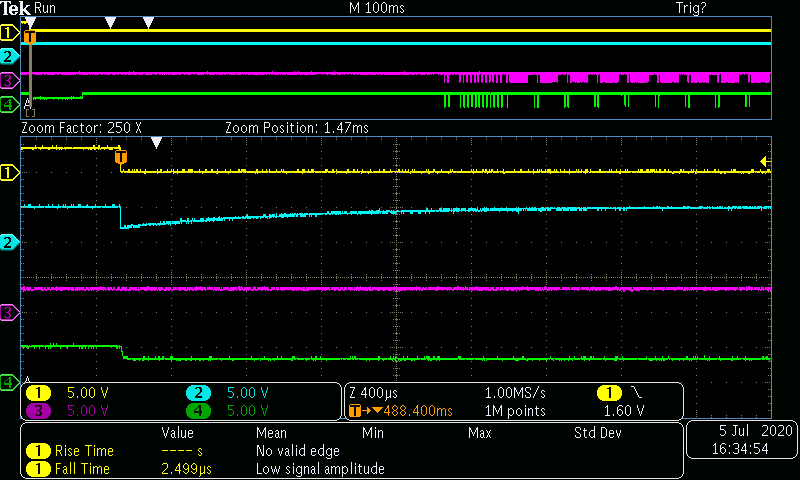
\includegraphics[width =  \textwidth]{graphics/ATMega2560_DTR_RESET_RX_TX_1}
\caption{Handshake zum Hochladen des Programmcodes auf den ATMega2560. Zoom auf den Moment des Resets.\\\hspace{\textwidth}1: Gelb = DTR; 2: Blau = Reset; 3: Violett = RX; 4: Grün = TX}
\label{fig:ATMega2560_DTR_RESET_RX_TX_1}
\end{figure}


\subsection{ESP32}\label{Appendix:Handshake_ESP}

\subsubsection{Wiring}\label{Appendix:Handshake_ESP_wiring}
\begin{table}[H]
\center
\begin{tabular}{|c|lcl|c|}
\hline
\textbf{ESP} & & & & \textbf{USB-Flash-Device} \\ \hline
RX & <== & direkt & === & TX  \\
TX & === & direkt & ==> & RX  \\
EN & <== & über Transistor & === & RTS \\
IO\_0 & <== & über Transistor & === & DTR \\
IO\_13 & <== & über Widerstand & === & RTS \\
IO\_15 & <== & über Widerstand & === & CTS \\
\hline
\end{tabular}
\caption{Verbindung zwischen USB und ESP.}
\label{tab:USB_ESP}
\end{table}

\subsubsection{Handshake}\label{Appendix:Handshake_ESP_Messung}

\begin{figure}[H]
	\centering
	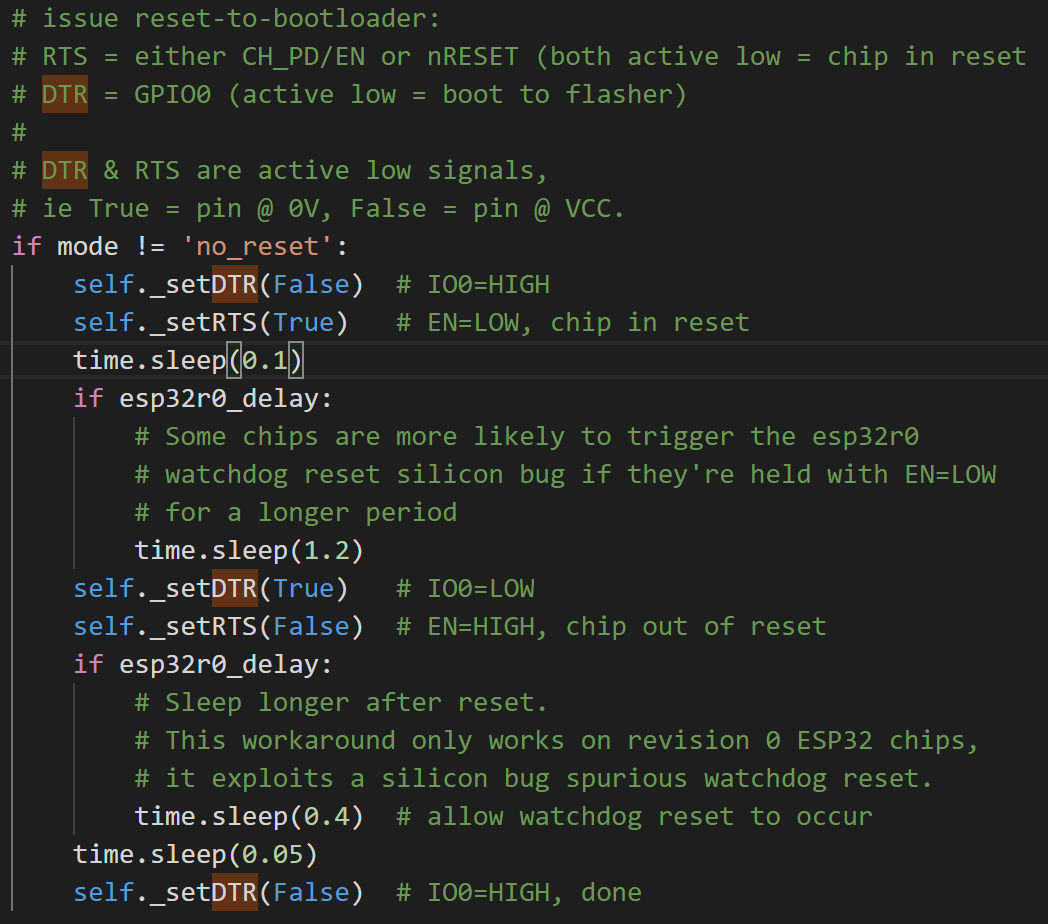
\includegraphics[width=0.8\textwidth]{graphics/ESP32_Boot_Code}
	\caption{Codeausschnitt aus dem Programmier-Tool. Auf diese Weise werden der DTR- und der RTS-Pin angesteuert während dem Programmiervorgang.}
	\label{fig:ESP32_Boot_Code}
\end{figure}

\begin{table}[H]
\center
\begin{tabularx}{\textwidth}{|l|X||c|c||c|c|}
\hline
Schritt & Beschreibung & DTR & RTS & EN & IO0\\
\hline
1 & Im ersten Schritt wird der Chip mit \textit{EN = 0} und \textit{IO0 = 1} in den Reset-Modus geschaltet und im Programm 0.1ms gewartet. & 1 & 0 & 0 & 1 \\
\hline
2 & Im zweiten Schritt werden die Zustände geändert, jetzt ist \textit{EN = 1} und \textit{IO0 = 0} \textit{IO0 = 0}. Aufgrund der Kapazität am EN-Pin wird die Spannung für einen kurzen Moment tief gehalten. Dies hat Schritt 3 zur Folge. & 0 & 1 & 1 & 0 \\
\hline
3 & Die durch den Kondensator C7 tief gehaltene Spannung bewirkt, dass sich die Zustsände über den Pins wie folgt verhalten: \textit{EN = 0} und \textit{IO0 = 0}. Im Programm wird 0.05ms gewartet. Danach ist das ESP32 im Download-Boot-Modus und das zu speichernde Programm kann hochgeladen werden. & 0 & 1 & 0 & 0 \\
\hline
4 & Nachdem das Programm hochgeladen wurde, werden beide Zustände auf 1 gesetzt. Das ESP32 startet nun den neu hochgeladenen Programmcode. & 1 & 1 & 1 & 1 \\
\hline
\end{tabularx}
\caption{Abfolge der Schritte während dem Aufrufen des Download-Boot-Modus.}
\label{tab:Abfolge_Download_Boot_Modus}
\end{table}

\begin{figure}[H]
\center
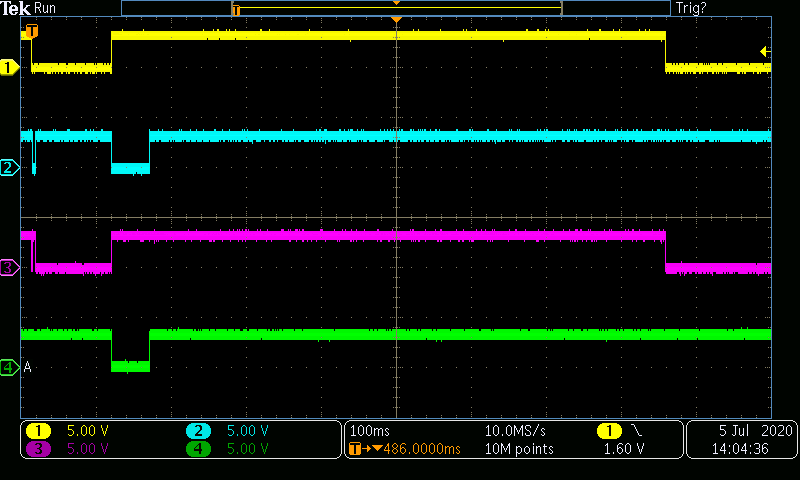
\includegraphics[width = \textwidth]{graphics/ESP32_RTS_DTR_EN_IO0_gesamt}
\caption{Handshake zum Hochladen des Programmcodes auf das ESP32. \\\hspace{\textwidth}1: Gelb = RTS; 2: Blau = DTR; 3: Violett = EN; 4: Grün = IO0;}
\label{fig:ESP32_RTS_DTR_EN_IO0_gesamt}
\end{figure}

\begin{figure}[H]
\center
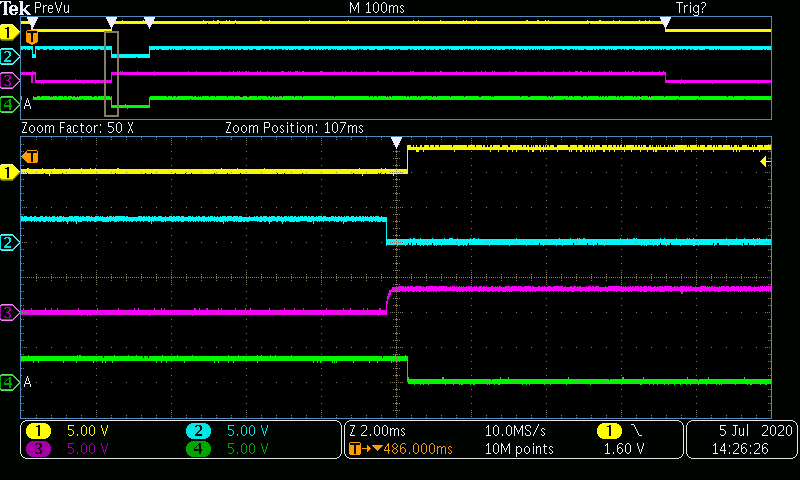
\includegraphics[width = 0.8\textwidth]{graphics/ESP32_RTS_DTR_EN_IO0_2}
\caption{Handshake zum Hochladen des Programmcodes auf das ESP32. Zoom auf gleichzeitiger Flankenwechsel RTS und DTR.\\\hspace{\textwidth}1: Gelb = RTS; 2: Blau = DTR; 3: Violett = EN; 4: Grün = IO0;}
\label{fig:ESP32_RTS_DTR_EN_IO0_2}
\end{figure}

\begin{figure}[H]
\center
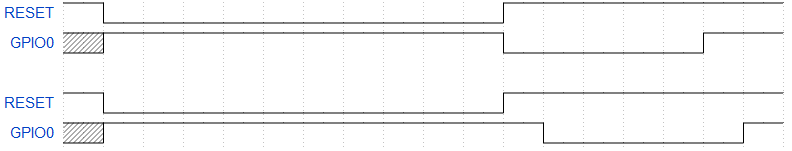
\includegraphics[width = 0.8\textwidth]{graphics/ESP32_Handshake_Forum}
\caption{Handshake zum Hochladen des Programmcodes auf das ESP32. Zoom auf gleichzeitiger Flankenwechsel RTS und DTR.}
\label{fig:ESP32_Handshake_Forum}
\end{figure}

\begin{figure}[H]
\center
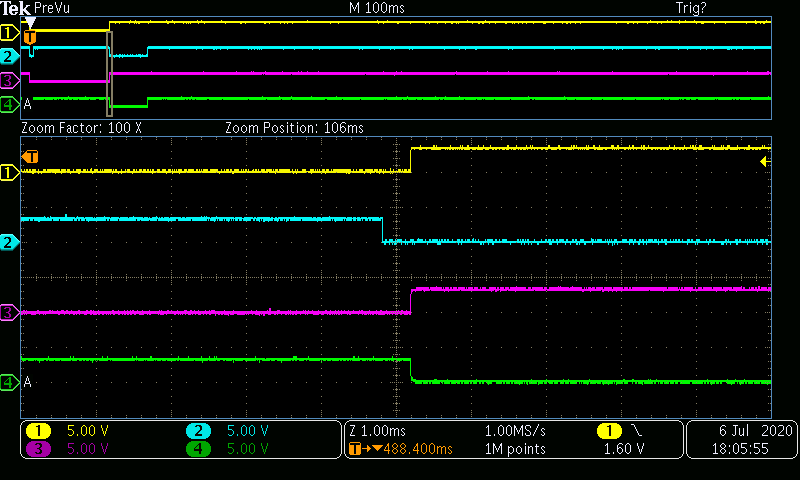
\includegraphics[width = 0.8\textwidth]{graphics/ESP32_RTS_DTR_EN_IO0_mit_Bruecke_1}
\caption{Handshake zum Hochladen des Programmcodes auf das ESP32. Zoom auf gleichzeitiger Flankenwechsel RTS und DTR.}
\label{fig:ESP32_RTS_DTR_EN_IO0_mit_Bruecke_1}
\end{figure}

In einem Forum\footnote{https://forum.micropython.org/viewtopic.php?t=4607} wurde diese Auffälligkeit, welche in Kapitel \ref{subsubsec:Inbetriebnahme_USB-B} erwähnt wurde, auch schon besprochen. Die Diskussion führte zum selben Ergebnis wie bei Inbetriebnahme. Nämlich, dass es nach dem Reset eine Zeit dauert, bis im Startprozess die Pins geprüft werden. Dazu gehört auch der Pin IO0. Somit ist es möglich, den Pin IO0 kurz nach dem Reset auf 0 zu ziehen.
Im selben Forum wurde auch die in Abbildung \ref{fig:ESP32_Handshake_Forum} gezeigte Darstellung gefunden. Ein Kommentar weist darauf hin, das mit dem esptool.py der EN-Pin des ESP32 direkt auf RTS gehängt werden kann. So lassen sich die Zeitpunkte, zu der die Pins auf 0 sind, näher zusammenschieben.

Die Messung nach dem Einlöten der Brücke bestätigt dies. Abbildung \ref{fig:ESP32_RTS_DTR_EN_IO0_mit_Bruecke_1} zeigt, dass das Umschalten von EN und GPIO0 gleichzeitig passiert. Allerdings spielt der Kondensator jetzt nicht mehr so eine grosse Rolle, was auch nicht nötig ist. Auf das Hochladen des Codes hat die Brücke keinen Einfluss. Die Funktioniert wie bei der Schaltung ohne Brücke einwandfrei.
